\chapter{Sistema Embebido}
\cleanchapterquote{I do not fear computers. I fear lack of them.}{Isaac Asimov}{(American writer and professor of biochemistry)}

\section{Sistema fisico}
El sistema físico de la gimbal fue hecho en colaboración con el alumno "Nombre" perteneciente
a la Universidad Aeronáutica en Querétaro. Dicho trabajo es detallado en seguida.\\
La idea de tener un sistema mecánico con dos ejes de libertad capaz de mover una cámara
es una tarea retadora, debido a que no se puede hacer de cualquier material ya que
los motores podrían no soportar el peso y no tener el torque necesario para mover la
estructura, por eso mismo se decidió por hacer una impresión 3D.
\begin{center}
	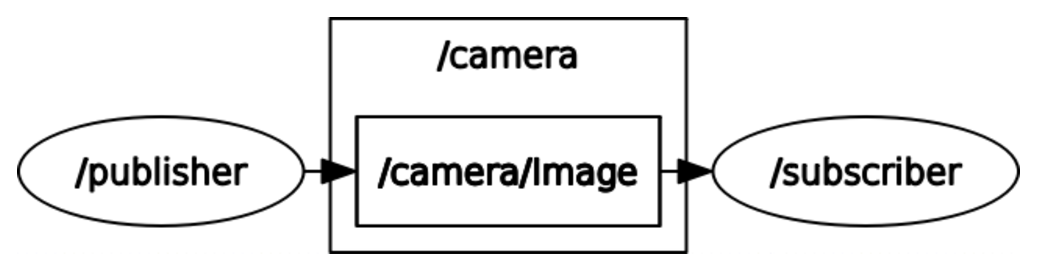
\includegraphics[width=0.5\textwidth]{Contenido/Cuerpo/Capitulo5/Fig0.eps}
	\captionof{figure}{CAD del sistema gimbal}\label{Fig1}
\end{center}
La imagen superior ilustra desde diferentes ángulos el ensamble de todas las piezas que
conforman al sistema mecánico.